\documentclass[11pt,a4paper]{article}
\usepackage[T1]{fontenc}
\usepackage[margin=2.3cm]{geometry}
\usepackage{amsmath,amssymb}
\usepackage{graphicx}
\usepackage[dvipsnames]{xcolor}
\usepackage{enumitem}
\usepackage[colorlinks=true,linkcolor=blue,urlcolor=blue]{hyperref}
\setlength{\parskip}{0.6em}
\setlength{\parindent}{0pt}
\begin{document}

\begin{center}{\LARGE\bfseries opensurvey}\\[0.4em]{\large Level a site and measure it with a total station model, in three sessions.}\\[0.2em]\small PAN IIT OSS explainer \textbullet{} diploma / undergraduate to advanced undergraduate (levels 5-6)\end{center}

\section*{Why this exists}
Every road, drain and building starts with measurements of angles, distances and heights. This explainer shows the mathematics behind that work, from a single staff reading to an adjusted closed traverse, using only subtraction, trigonometry and a little statistics.

\section*{The end goal}
Level a site and measure distances with trigonometry and a total station model. The end goal is to level a site and measure it with a total station model: reduce a levelling book, turn slope distances and bearings into coordinates, and close, adjust and test a traverse. The same ideas are used in construction setting-out and in mapping, and every model here is a simplified teaching model, not a tool for legal or construction work.

\section*{How the three sessions build up}
\begin{enumerate}[nosep]
\item \textbf{Session 1: Height difference with a level and a staff} (Level 1, conceptual interactive model, 60 min).
\item \textbf{Session 2: Levelling books, slope distances and total-station coordinates} (Level 2, mathematical engineering model, 75 min).
\item \textbf{Session 3: Close, adjust and test a traverse} (Level 3, simulation and validation, 90 min).
\end{enumerate}

\section{Session 1: Height difference with a level and a staff}

\subsection*{A. Real-world problem}
Before a road, a drain or a building platform is built, someone must know how much higher or lower one point is than another. Water only runs downhill, so a drain that slopes the wrong way does not work. You cannot tell by eye. A surveyor uses a level (a telescope that stays exactly horizontal) and a staff (a tall ruler held upright) and subtracts two readings. How can two readings, taken from a spot that is neither point, give the height difference between them?

\subsection*{B. Concept and theory}
The level is set up between two points A and B. Its line of sight is perfectly horizontal at some height above the datum (the reference height, such as sea level). The staff is held upright on A and read through the telescope: that is the backsight, bs. Then the staff is moved to B: that is the foresight, fs. A large reading means the ground is low, because most of the staff is then below the line of sight. So the rise from A to B is bs - fs (a negative answer is a fall), and the reduced level (RL, the height above the datum) of B is the RL of A plus that rise. If B is too far for one set-up, the surveyor leaves the staff on a turning point and moves the level on. Distance can be found roughly by pacing: walk a known distance, count paces, and use distance = paces x pace length.

\begin{itemize}[nosep]
\item bs: backsight: staff reading on the point behind (the known point) (m)
\item fs: foresight: staff reading on the point ahead (m)
\item RL: reduced level: height above the chosen datum (m)
\item HI: height of the line of sight (collimation height) (m)
\item pace length: average length of one pace, from a calibration walk (m)
\end{itemize}

\begin{equation*}
\text{rise from A to B}=bs-fs,\qquad RL_B=RL_A+(bs-fs)
\end{equation*}

\begin{equation*}
bs=HI-RL_A,\quad fs=HI-RL_B\ \Rightarrow\ bs-fs=RL_B-RL_A\ \text{(HI cancels)}
\end{equation*}

\begin{equation*}
\text{distance}=\text{paces}\times\text{pace length}
\end{equation*}

\begin{center}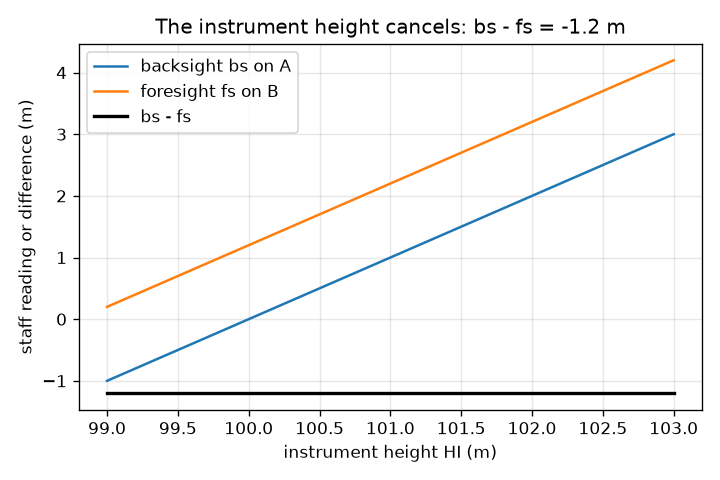
\includegraphics[width=0.85\linewidth]{figures/s01_height_cancels.png}\\\small Backsight and foresight change with the instrument height; their difference does not.\end{center}

\subsection*{E. Worked example}
A benchmark A has RL 100.000 m. The backsight on A is 1.525 m and the foresight on B is 2.310 m. Find the rise or fall and the RL of B.
\begin{enumerate}[nosep]
\item Rise = bs - fs = 1.525 - 2.310 = -0.785 m.
\item The negative sign means a fall: B is 0.785 m lower than A.
\item RL of B = 100.000 + (-0.785) = 99.215 m.
\item Sanity check: the foresight is bigger than the backsight, so the staff on B is lower in the line of sight, so B is the lower point. The answer is consistent.
\end{enumerate}
\textbf{Answer.} B is 0.785 m lower than A, at RL 99.215 m.

\subsection*{F. Questions}
\begin{enumerate}[nosep]
\item \textbf{Conceptual.} Why does the answer bs - fs not depend on how high the level is above the ground?
\item \textbf{Numerical.} The backsight on a point of RL 54.320 m is 0.872 m and the foresight on the next point is 2.134 m. Find the RL of the next point and say whether the ground rises or falls.
\item \textbf{Graph and simulation interpretation.} From the levelling-run figure, what is the grade (slope in percent) of the ground, and how much does it fall per set-up?
\item \textbf{Design and optimisation challenge.} Design: the staff is 4.0 m long, the ground falls 5 percent from the backsight staff, and the backsight reads 1.0 m. How far away can the foresight staff stand so that the reading is still on the staff? Why not simply use very short sights?
\end{enumerate}

\section{Session 2: Levelling books, slope distances and total-station coordinates}

\subsection*{A. Real-world problem}
A real levelling run is written in a table, the levelling book, and a single wrong subtraction spoils every level after it. A total station, the instrument that has replaced the theodolite and tape on many sites, measures a slope distance and angles, and a computer must turn those into coordinates on a map. And a practical question: over 1 km of levelling, how far apart can the staffs stand if small random reading errors of 2 mm per set-up must add up to less than 10 mm?

\subsection*{B. Concept and theory}
In a levelling book each row is a backsight (BS), an intermediate sight (IS) or a foresight (FS). A foresight followed by a backsight is a change point: the same point seen from two set-ups. Height of instrument method: at each set-up, HI = RL of the backsight point + BS, and every other point has RL = HI - reading. Rise and fall method: compare each reading with the one before it in the same set-up; rise = previous - current; RL = previous RL + rise. Both must give the same levels. The arithmetic check says: sum of backsights - sum of foresights = last RL - first RL. It checks the arithmetic of the chain, not the readings, and it cannot see a wrong intermediate sight. For a total station, the slope distance S and the elevation angle a give the horizontal distance D = S cos a and the height change V = S sin a. From a station at (E0, N0), with the bearing measured clockwise from north, a point at horizontal distance D is at E = E0 + D sin(bearing) and N = N0 + D cos(bearing). Finally, random errors do not add up in a straight line: if each of n set-ups adds an independent error with standard deviation s, the total has standard deviation s sqrt(n).

\begin{itemize}[nosep]
\item BS, IS, FS: backsight, intermediate sight, foresight readings (m)
\item HI: height of instrument (collimation height) (m)
\item S: slope distance measured by the total station (m)
\item a: elevation angle above the horizontal (degrees)
\item D, V: horizontal distance and height change (m)
\item bearing: direction, clockwise from grid north (degrees)
\item E, N: easting and northing (grid coordinates) (m)
\item s: standard deviation of the error of one set-up (mm)
\item n: number of set-ups (no unit)
\end{itemize}

\begin{equation*}
HI=RL_{\text{back}}+BS,\qquad RL=HI-\text{reading}
\end{equation*}

\begin{equation*}
\text{rise}=\text{previous reading}-\text{current reading},\qquad RL=RL_{\text{previous}}+\text{rise}
\end{equation*}

\begin{equation*}
\sum BS-\sum FS=RL_{\text{last}}-RL_{\text{first}}
\end{equation*}

\begin{equation*}
D=S\cos a,\qquad V=S\sin a
\end{equation*}

\begin{equation*}
E=E_0+D\sin\beta,\qquad N=N_0+D\cos\beta
\end{equation*}

\begin{equation*}
\sigma_n=s\sqrt{n},\qquad n<\left(\dfrac{\text{limit}}{s}\right)^2
\end{equation*}

\begin{center}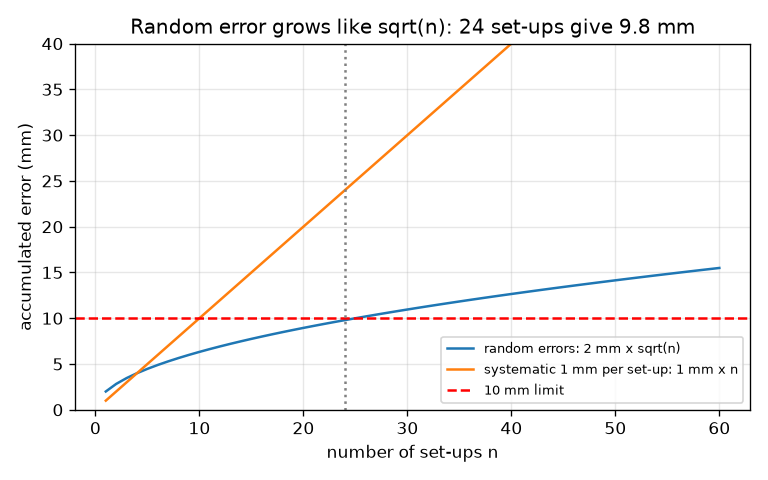
\includegraphics[width=0.85\linewidth]{figures/s02_error_growth.png}\\\small Random error grows like sqrt(n); a systematic error grows like n.\end{center}

\subsection*{E. Worked example}
Reduce the levelling book of the lesson (BS 1.425 on a benchmark of RL 100.000, IS 1.870, IS 2.315, FS 2.905, then BS 1.150, IS 0.980, FS 0.640). Then a total station at E 1000.000, N 5000.000, RL 50.000, with instrument height 1.55 m, measures a prism (height 1.80 m) at slope distance 85.340 m, elevation angle 7.5 degrees, bearing 63.5 degrees. Find the coordinates and the RL.
\begin{enumerate}[nosep]
\item First set-up: HI = 100.000 + 1.425 = 101.425 m. Levels: 101.425 - 1.870 = 99.555, 101.425 - 2.315 = 99.110, 101.425 - 2.905 = 98.520 m (the change point).
\item Second set-up: HI = 98.520 + 1.150 = 99.670 m. Levels: 99.670 - 0.980 = 98.690 and 99.670 - 0.640 = 99.030 m.
\item Rise and fall gives the same: the first intermediate sight is a fall of 1.425 - 1.870 = -0.445 m, and so on.
\item Arithmetic check: sum BS = 2.575, sum FS = 3.545, difference -0.970. Last RL - first RL = 99.030 - 100.000 = -0.970. They agree.
\item Total station: D = 85.340 cos 7.5 degrees = 84.610 m and V = 85.340 sin 7.5 degrees = 11.139 m (use the program for the digits).
\item E = 1000 + 84.610 sin 63.5 degrees = 1075.720 and N = 5000 + 84.610 cos 63.5 degrees = 5037.753.
\item RL of the ground at the prism = 50.000 + 1.55 + V - 1.80 = 60.889 m.
\end{enumerate}
\textbf{Answer.} Levels 99.555, 99.110, 98.520, 98.690 and 99.030 m (check passed); the point is at E 1075.720, N 5037.753, RL 60.889 m, and the inverse from the station returns bearing 63.5 degrees and distance 84.610 m.

\subsection*{F. Questions}
\begin{enumerate}[nosep]
\item \textbf{Conceptual.} A student adds a misread intermediate sight (0.100 m too big) to the levelling book and finds the arithmetic check still passes. Is the check useless? What does it prove and what does it not?
\item \textbf{Numerical.} A tape along a slope reads S = 120.50 m at an elevation angle of 12 degrees. Find D and V. Then, from E 1000, N 5000, find the point 50 m away at bearing 245 degrees.
\item \textbf{Graph and simulation interpretation.} In the graph of D and V against the angle for S = 100 m, how much shorter than S is D at 10 degrees and at 25 degrees? What does this say about when you can ignore the slope?
\item \textbf{Design and optimisation challenge.} Design: a 4 km levelling line must have a random error below 10 mm, and each set-up has s = 1.5 mm. How many set-ups at most, and what spacing is that? Choose a practical spacing of whole tens of metres and give the resulting error. Mention one other limit on the spacing.
\end{enumerate}

\section{Session 3: Close, adjust and test a traverse}

\subsection*{A. Real-world problem}
To fix the corners of a plot, a surveyor walks round it: the angle at each corner and the length of each side are measured. Because every measurement has a small error, the walk does not quite end where it began. How big is that gap, is it acceptable, and how should it be spread over the corners? And the nasty case: what if one angle is simply read wrongly, and the tidy adjustment makes the figure close perfectly anyway?

\subsection*{B. Concept and theory}
A closed traverse has n corners. From the bearing of the first leg and the interior angles (walking clockwise), each next bearing is the previous bearing + 180 - interior angle. Each leg of length D and bearing b contributes a departure dE = D sin b and a latitude dN = D cos b. For a perfect traverse, the sum of all departures and the sum of all latitudes are zero. In practice their sums (eE, eN) are the misclosure vector; its length is the misclosure. The relative accuracy is perimeter / misclosure, written 1 in N (1 in 5000 is a commonly used target for ordinary work). The interior angles of an n-sided polygon sum to (n - 2) x 180 degrees: any difference is the angular misclosure, shared equally between the angles first. The Bowditch (compass) rule then gives leg i a correction proportional to its length: cE\_i = -eE D\_i / P and cN\_i = -eN D\_i / P, where P is the perimeter. These corrections sum to exactly -e, so the adjusted traverse closes exactly. The area follows from the corner coordinates by the shoelace formula. Errors are studied by simulation: add random errors to a known polygon (typical figures for a mid-range total station: 20 arc-seconds per angle, and 5 mm + 5 ppm per distance), adjust, and compare with the exact answer, many times. For long sights, the Earth's curvature and the bending of light matter: the combined correction to a staff reading is about 0.0675 K\textasciicircum{}2 metres for a sight of K kilometres.

\begin{itemize}[nosep]
\item D, b: leg length and bearing (m, degrees)
\item dE, dN: departure and latitude of a leg (m)
\item eE, eN: misclosure vector (sum of departures, sum of latitudes) (m)
\item P: perimeter (sum of leg lengths) (m)
\item 1 in N: relative accuracy, N = P / misclosure (no unit)
\item sigma: standard deviation of a measurement (typical: 20 arc-seconds; 5 mm + 5 ppm) (arc-seconds, mm)
\item K: length of a long sight (km)
\item k: coefficient of refraction (typical 0.14) (no unit)
\item R: radius of the Earth, 6371 km (km)
\end{itemize}

\begin{equation*}
b_{i}=b_{i-1}+180^\circ-\theta_i,\qquad dE_i=D_i\sin b_i,\quad dN_i=D_i\cos b_i
\end{equation*}

\begin{equation*}
e_E=\sum dE_i,\quad e_N=\sum dN_i,\quad e=\sqrt{e_E^2+e_N^2},\quad \text{1 in }N,\ N=P/e
\end{equation*}

\begin{equation*}
\sum\theta_i=(n-2)\times180^\circ
\end{equation*}

\begin{equation*}
c_{E,i}=-e_E\,\frac{D_i}{P},\quad c_{N,i}=-e_N\,\frac{D_i}{P},\quad \sum_i(dE_i+c_{E,i})=0
\end{equation*}

\begin{equation*}
A=\tfrac12\left|\sum_i\left(E_iN_{i+1}-E_{i+1}N_i\right)\right|
\end{equation*}

\begin{equation*}
c\approx\frac{(1-k)K^2}{2R}\approx0.0675\,K^2\ \text{m}
\end{equation*}

\begin{center}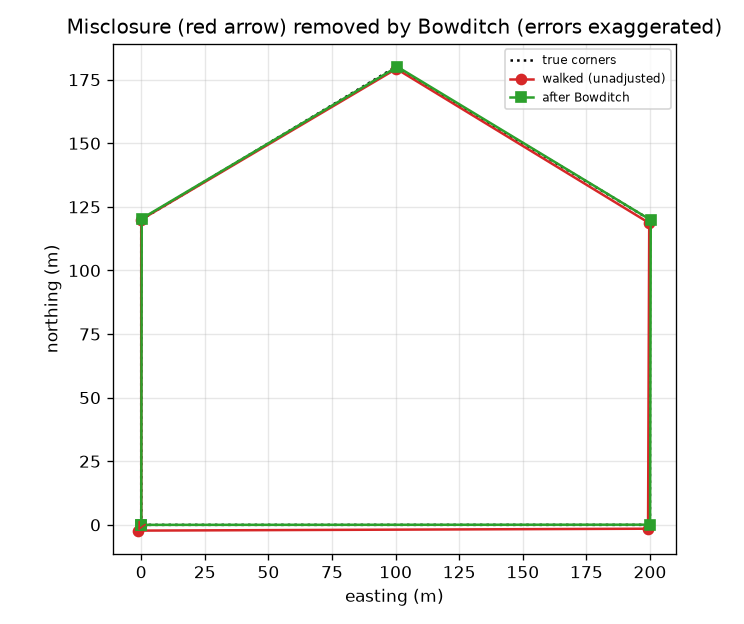
\includegraphics[width=0.85\linewidth]{figures/s03_bowditch.png}\\\small A walked traverse with exaggerated errors: misclosure (red arrow) and the Bowditch-adjusted closed figure (green).\end{center}

\subsection*{E. Worked example}
A traverse of perimeter 673.238 m has a misclosure vector (eE, eN) = (+0.100, -0.060) m. Find the misclosure, the relative accuracy, and the Bowditch correction for the 200 m leg. Is 1 in 5000 met?
\begin{enumerate}[nosep]
\item Misclosure = sqrt(0.100\textasciicircum{}2 + 0.060\textasciicircum{}2) = 0.1166 m.
\item Relative accuracy = 673.238 / 0.1166 = 5773, so 1 in 5773.
\item The 200 m leg gets cE = -0.100 x 200 / 673.238 = -0.0297 m and cN = +0.060 x 200 / 673.238 = +0.0178 m.
\item 1 in 5773 is better than 1 in 5000, so the traverse is acceptable and may be adjusted.
\item The five corrections for all legs sum to (-0.100, +0.060), the opposite of the misclosure, so the adjusted traverse closes exactly (the checkpoint verifies this on a simulated survey).
\item Area check on the exact plot (rectangle 200 m x 120 m plus a gable of base 200 m and height 60 m): 24000 + 6000 = 30000 m2, and the shoelace formula gives the same.
\end{enumerate}
\textbf{Answer.} Misclosure 0.1166 m, relative accuracy 1 in 5773 (acceptable); the 200 m leg is corrected by (-0.0297, +0.0178) m; the plot area is 30000 m2.

\subsection*{F. Questions}
\begin{enumerate}[nosep]
\item \textbf{Conceptual.} The Bowditch rule always makes a traverse close exactly. Does a perfect closure after adjustment prove that the survey is correct? Give an example from this session.
\item \textbf{Numerical.} A traverse of 673.238 m perimeter closes with a misclosure of 0.050 m. What is the relative accuracy? How much is a leg of 116.619 m corrected?
\item \textbf{Graph and simulation interpretation.} Read the sensitivity graph: roughly how large can the angle error become before the typical misclosure exceeds the 1 in 5000 limit? What does the straight rise tell you about the effect of a better instrument?
\item \textbf{Design and optimisation challenge.} Design: choose the poorest angle standard deviation (in arc-seconds) so that about 95 percent of surveys of this plot meet 1 in 5000. Hint: require the RMS misclosure to be at most half the limit. Why half, and what is the trade-off?
\end{enumerate}

\section{Real-world mini-project}
\textbf{Adjust a field traverse and report coordinates and area.} A crew hands you the synthetic field book of a six-corner site, walked clockwise from corner 1 at E 5000.000, N 10000.000 m (\texttt{FIELD\_START}, \texttt{FIELD\_B0}, \texttt{FIELD\_ANGLES}, \texttt{FIELD\_DISTS} in Session 3). The angles do not add up: one of them was misread. Run the angle check and the adjustment as given, find the corner with the blunder using \texttt{locate\_angle\_blunder}, correct that angle, adjust again, and report the final corner coordinates and the area.

\section{The path ahead}
\begin{enumerate}[nosep]
\item \textbf{Session 4: Least-squares adjustment.} A second adjustment function that estimates the corner coordinates by weighted least squares and reports the residuals.
\item \textbf{Session 5: Find distance blunders too.} A locator for the leg with a distance blunder, using the direction of the misclosure vector.
\item \textbf{Session 6: A levelling network.} A loop of four levelling lines with known benchmark levels, adjusted so that every loop closes.
\item \textbf{Session 7: Resection: where am I?.} A function that solves the coordinates of an unknown station from the angles measured to three known points, with a picture of the geometry.
\item \textbf{Session 8: Contours and earthwork.} A grid of levels, contour lines, and the volume to cut and fill to make a level platform.
\end{enumerate}

\section{Answers and hints}

\subsection*{Session 1}
\begin{enumerate}[nosep]
\item \textbf{Conceptual.} Hint: Write each reading as the height of the line of sight minus the height of the ground. Solution: bs = HI - RL\_A and fs = HI - RL\_B, so bs - fs = RL\_B - RL\_A: HI cancels. If the instrument is raised by 0.40 m, both readings drop by 0.40 m and the difference is unchanged (-1.2 m in the run of the lesson). That is why the level can stand anywhere between the two staffs.
\item \textbf{Numerical.} Hint: Rise = bs - fs, then add to the RL. Solution: Rise = 0.872 - 2.134 = -1.262 m, a fall. RL = 54.320 - 1.262 = 53.058 m. Sanity check: the foresight is bigger, so the new point is lower. Units: metres.
\item \textbf{Graph and simulation interpretation.} Hint: Grade = fall divided by horizontal distance, times 100. Solution: The ground falls 3.6 m over 90 m, so the grade is 3.6 / 90 x 100 = 4 percent. Each of the three set-ups covers 30 m and falls 1.2 m, the same each time because the slope is uniform.
\item \textbf{Design and optimisation challenge.} Hint: The foresight is the backsight plus the fall over the distance. Solution: fs = 1.0 + 0.05 x d must stay at or below 4.0 m, so d is at most 60 m. Very short sights need more set-ups for the same line, so more readings, more time and more chances for small errors to add up (Session 2 shows how fast). A good plan uses the longest sights that stay on the staff and within the telescope's reliable range, and keeps backsight and foresight lengths about equal.
\end{enumerate}

\subsection*{Session 2}
\begin{enumerate}[nosep]
\item \textbf{Conceptual.} Hint: Which readings feed the last RL? Solution: The check compares sum BS - sum FS with the last RL minus the first RL. Intermediate sights appear in neither, so a wrong IS leaves the check passing while that point's own level is wrong by 0.100 m. The check proves the reductions along the backsight and foresight chain were done without an arithmetic slip (a slip of 0.010 m in the last level would break it). It does not prove that the readings were read or booked correctly. Intermediate sights need a different check, such as a closing line or a second reading.
\item \textbf{Numerical.} Hint: D = S cos a, V = S sin a; then E = E0 + D sin(bearing), N = N0 + D cos(bearing). Solution: D = 120.50 cos 12 = 117.87 m and V = 120.50 sin 12 = 25.05 m. Sanity check: D is a little less than S and V is about 0.2 of S, which fits 12 degrees. For the point: E = 1000 + 50 sin 245 = 954.68 and N = 5000 + 50 cos 245 = 4978.87 (south-west of the station, which is right for 245 degrees). Units: metres.
\item \textbf{Graph and simulation interpretation.} Hint: Compute 1 - cos a for each angle. Solution: D is S cos a, so the shortening is 1 - cos a: 1.5 percent at 10 degrees (1.5 m in 100 m) and 9.4 percent at 25 degrees. On gentle slopes the correction is small but it is never zero; for work to a few millimetres per 100 m it must always be applied. The curve is flat near 0 degrees because the cosine is flat there.
\item \textbf{Design and optimisation challenge.} Hint: n \textless{} (limit / s)\textasciicircum{}2, spacing = length / n. Solution: n \textless{} (10 / 1.5)\textasciicircum{}2 = 44.4, so at most 44 set-ups: the spacing must be at least 4000 / 44 = 90.9 m. A practical choice is 100 m, which means 40 set-ups and an error of 1.5 x sqrt(40) = 9.49 mm, inside the limit. The other limit is the other direction: the staff must still be readable and the line of sight must not be too close to the ground, so very long sights are not allowed, and curvature and refraction (Session 3) grow as the square of the sight length. Trade-off: fewer, longer set-ups are faster and accumulate less random error but are limited by visibility and by the Earth's curvature.
\end{enumerate}

\subsection*{Session 3}
\begin{enumerate}[nosep]
\item \textbf{Conceptual.} Hint: Think about what the rule does to a blunder. Solution: No. The rule forces the figure to close whatever the cause of the gap. In the lesson, one interior angle is read 1 degree too big. The raw misclosure is 4.071 m, and after spreading the angle error the misclosure is 1.851 m (1 in 364), yet after Bowditch the figure closes to better than 1e-9 m while the corners are wrong by up to 0.56 m and the area by about 10.5 m2. The quality is judged by the misclosure and the angle check before adjustment, not by the closure afterwards.
\item \textbf{Numerical.} Hint: N = P / misclosure; the correction is the misclosure component times D / P. Solution: Relative accuracy = 673.238 / 0.050 = 13465, so 1 in 13465, well inside 1 in 5000. For a leg of 116.619 m the share of the misclosure is 116.619 / 673.238 = 0.173, so the total correction is 0.050 x 0.173 = 0.0087 m (split between east and north in proportion to the misclosure components). Units: metres.
\item \textbf{Graph and simulation interpretation.} Hint: Compare the values at 40 and 80 arc-seconds with 134.6 mm. Solution: At 40 arc-seconds the RMS misclosure is about 76 mm, inside the limit of 134.6 mm; at 80 arc-seconds it is about 149 mm, outside. The crossing is at about 71 arc-seconds. Above about 40 arc-seconds, doubling the angle error doubles the misclosure (76, 149 and 298 mm at 40, 80 and 160 arc-seconds): halving the angle error roughly halves it. A distance part of about 13 mm remains whatever the angle quality, so improving the angles beyond a point brings less and less.
\item \textbf{Design and optimisation challenge.} Hint: Use max\_angle\_sigma(limit / 2), then check the pass rate with monte\_carlo. Solution: The limit is 673.238 / 5000 = 0.1346 m. A random 2D error is within about twice its RMS in nearly all cases, so require RMS at most 0.0673 m. The program gives 35 arc-seconds. The Monte Carlo pass rate is about 97 percent at 35 arc-seconds and 94 percent at 40, so 35 is the safe choice. If you accepted an RMS equal to the limit (71 arc-seconds), many surveys would fail: at 80 arc-seconds only about 58 percent pass. Trade-off: a 5 arc-second instrument costs far more than a 30 arc-second one, but a failed survey means walking the traverse again. Assumption: the errors are random with the typical distance quality; a blunder is not covered by any instrument grade.
\end{enumerate}

\section{How to join}
Read \texttt{CONTRIBUTING.md} in the repository, then pick an issue labelled \texttt{good first issue}. Repository: \url{https://github.com/KrunalPanchal1995/opensurvey}

\end{document}
